\chapter{相关理论与技术}

% 这是一个示例章节，展示了各级标题、图片、表格、公式、算法等的使用方法
% 请根据你的论文内容修改章名和内容

\section{二级标题示例}

正文内容使用小四号宋体，首行缩进2字符。外文和数字使用 Times New Roman 字体。

分段时空一行即可。

\subsection{三级标题示例}

三级标题使用四号黑体。

\subsubsection{四级标题示例}

四级标题使用小四号黑体，在此之下若需分级可用（1）、（2）等形式。

%% ============================================================
%% 插图示例
%% ============================================================
\section{插图示例}

图号采用章序号编码，如图\ref{fig:example}所示。图题置于图的正下方，使用5号字。

\begin{figure}[htbp]
    \centering
    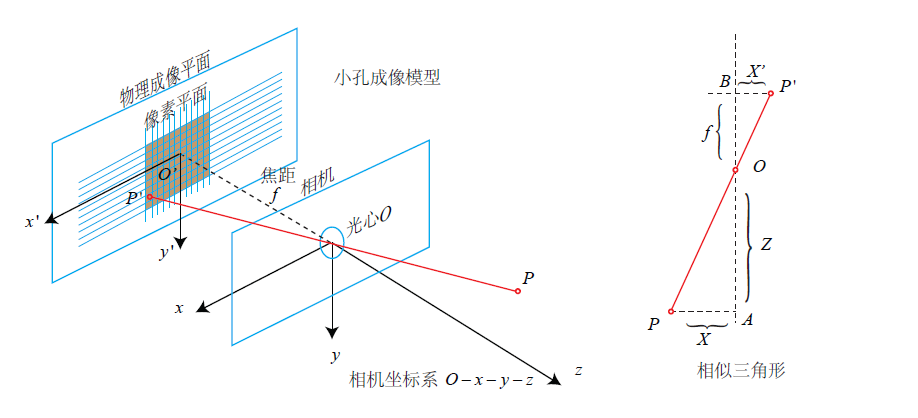
\includegraphics[width=0.8\textwidth]{images/slam-01.png}
    \caption{示例图片标题}
    \label{fig:example}
\end{figure}

%% ============================================================
%% 表格示例
%% ============================================================
\section{表格示例}

表号也用章序号编码，如表\ref{tab:example}。表题置于表的上方居中。

\begin{table}[htbp]
    \centering
    \caption{示例三线表}
    \label{tab:example}
    \begin{tabular}{lccc}
        \toprule
        名称 & 参数1 & 参数2 & 参数3 \\
        \midrule
        方法A & 0.95 & 0.87 & 0.92 \\
        方法B & 0.91 & 0.89 & 0.90 \\
        方法C & 0.93 & 0.91 & 0.94 \\
        \bottomrule
    \end{tabular}
\end{table}

%% ============================================================
%% 公式示例
%% ============================================================
\section{公式示例}

公式按章序号编号，如式(\ref{eq:example})。公式单行居中排版，式号居右。

\begin{equation}
    E = mc^2
    \label{eq:example}
\end{equation}

其中，$E$为能量，$m$为质量，$c$为光速。

%% ============================================================
%% 算法示例
%% ============================================================
\section{算法示例}

\begin{algorithm}[htbp]
    \caption{示例算法}
    \label{alg:example}
    \begin{algorithmic}[1]
        \Require 输入数据 $X$
        \Ensure 输出结果 $Y$
        \State 初始化参数
        \For{$i \leftarrow 1$ to $n$}
            \State 计算 $f(x_i)$
            \If{$f(x_i) > \theta$}
                \State 更新 $Y$
            \EndIf
        \EndFor
        \State \Return $Y$
    \end{algorithmic}
\end{algorithm}
